\documentclass[conference]{IEEEtran}
\IEEEoverridecommandlockouts
% The preceding line is only needed to identify funding in the first footnote. If that is unneeded, please comment it out.
\usepackage{cite}
\usepackage{amsmath,amssymb,amsfonts}
\usepackage{algorithmic}
\usepackage{graphicx}
\usepackage{textcomp}
\usepackage{xcolor}
\def\BibTeX{{\rm B\kern-.05em{\sc i\kern-.025em b}\kern-.08em
    T\kern-.1667em\lower.7ex\hbox{E}\kern-.125emX}}
\begin{document}

\title{Predict Solar Panel Power Production Using Weather Forecasts}

\author{\IEEEauthorblockN{Pankajan Satkunam}
\IEEEauthorblockA{\textit{Software Engineering Teaching Unit} \\
\textit{University of Kelaniya}\\
pankajan05@gmail.com}
}

\maketitle

\begin{abstract}
Renewable energy is the best solution for fossil fuels. Solar energy is widely used as a renewable energy source in the homes and the industries. Weather conditions are the major factor that affect solar power generation. Sri Lanka is close to the equator that receive more sunlight and is a tropical country that affected by the unpredictable weather conditions. In the Sri Lanka, there are many solar panel users who generate electricity for ordinary households and industrial energy. When the solar power energy generation decreases solar panel users must rely on fossil fuel energy. It increases the load in the main grid. 

This research focuses on how weather affects solar panel productivity and how users use the green energy-efficient way using accurate weather prediction systems. The weather data is collected from the Colombo airport and the solar panel energy production data is collected from CEB (Ceylon Electricity Board). Other than, Google form is distributed to the solar panel users and collect data about the weather prediction system that they are currently using for assume the weather conditions. First, The correlation is analyzed between weather and solar energy production. Then, this research discuss about how the weather prediction system can utilize to predict the solar panel power prediction. The research aims at converting the weather predictions system into a solar power prediction and use solar power efficiently and manage the load in the main grid.\\
\end{abstract}

\begin{IEEEkeywords}
Weather Prediction, Solar Energy Prediction, Weather Forecast, Data Analytic.
\end{IEEEkeywords}

\section{Introduction}
Climate change is one of the major issues in this world. Climate change affects many people's daily lives and costs many lives. \cite {ipcc} The Intergovernmental Panel on Climate Change (IPCC) found that in 2018, 89\% of global CO\textsubscript{2} gas emissions came from fossil fuels. Fossil fuels are one of the major reasons for climate change. \cite{iea} According to the International Energy Agency (IEA) fossil fuels like coal and natural gases are used in 60.19\% electricity generated in the world. Fossil fuel usage in electricity generation releases a large amount of CO\textsubscript{2} and other greenhouse gases into the atmosphere and contributes to global warming and climate change. Nuclear energy and renewable energy sources are the solutions for substituting fossil fuel usage in electricity generation.

\cite{iea} \cite{bp} 10.12\% of electricity produced in 2020 using nuclear energy. Nuclear energy causes environmental problems and produces 400,000 tons of nuclear waste per year worldwide, according to the World Nuclear Association. It is difficult and expensive to dispose of this nuclear waste. If this nuclear waste is released into the environment, then it is difficult to remove those radio-active particles from the environment. Natural disasters such as floods, tsunamis, and earthquakes could easily damage nuclear plants and cause the release of radioactive particles into the atmosphere. \cite{wna} Those radioactive particles take 1,000-10,000 years to decay. So, this nuclear plant energy could not be the best substitute for fossil fuels.

Renewable energy sources such as wind, solar, hydro, and geothermal energy could be used for electricity generation. Renewable energy is environmentally friendly and is renewable. \cite{bp} In 2020, around 28.97\% of the energy used in the world produced from renewable sources. \cite{bp} In the total renewable energy generation, 60.08\% of energy is generated from hydro-power. Only 10.3\% of energy is generated using solar power. We can increase the energy generated from solar power.



Countries close to the equator get more efficient solar energy than countries far from the equator. It happens because of the inclination of the earth's axis. \cite {geo} Sri Lanka is close to the equator and it is the 25th largest island, which has 65,612 km2 of land. Sri Lanka could use solar energy for electricity generation rather than fossil fuels. Sri Lanka is a tropical country that gets more rainfall and has very quickly changing weather conditions.



Sri Lanka is divided into the wet zone and dry zone according to the weather pattern and rainfall. The Western, Southwestern, and Central provinces fall into the wet zone, which receives an average of 2500 millimeters or more rainfall annually. The southwestern monsoon brings more rainfall to the wet zone. The Northern, Northwest, Southeast, and East country parts come into the dry zone, which annually gets between 600 and 1900 mm of rainfall\cite{geo}. The dry zone gets rain mostly from the northeast monsoon. The dry zone is better for solar energy generation because bad weather does not affect solar energy generation as much as it does in the wet zone. The weather conditions of the wet zone affect solar power generation.



Western Province is located in the wet zone and is one of the major cities and commercial capitals of Sri Lanka. Many solar panel users in the Western province have fixed solar panels on their home rooftops, and some industries also use solar panels to produce electricity. These solar panel users could not produce sufficient electricity during bad weather conditions or cloudy times. So, they rely on the main grid for electricity usage. When the solar panel users rely on the main grid load, the main grid will increase. It is mandatory to use the solar panel power generation prediction system to balance the load on the main grid.

The fuel crisis shut down fossil fuel electricity production in countries like Sri Lanka and European countries. Even the generators don't have the fuel to produce electricity. Even hospitals can't operate their medical electric equipment because of the power crisis in Sri Lanka in 2022. The solar panel systems can provide support at these times. The solar panel system can help to produce electricity for countries that have a fuel crisis. 

Currently, solar panel users directly use weather prediction systems to predict solar power generation. They directly depend on the mobile and web weather prediction systems and the weather forecast news. Experienced solar panel users could be able to predict the solar panel's power generation using weather prediction systems. The novice solar panel users can't predict the solar panel power production accurately using weather prediction systems. This research analysis shows how solar panel power generation is affected by weather conditions. The efficiency of the weather prediction system is analyzed to predict solar power generation. The Google form was distributed to the experienced solar panel users in Sri Lanka to confirm the usage of the weather predictions.



The specific objectives of this research paper are as follows:

\begin{itemize}

\item Analysis the relationship between weather conditions and solar power generation.

\item Analysis the efficiency of the weather prediction system to use to predict solar power generation.

\end{itemize}







\section{Related Research}

Renewable energy generation is uncontrollable and depends on weather conditions \cite{Hybrid}\cite{NavinSharma}\cite{Mohamed}\cite{Sam}. So users should depend on the grid. Solar power generation varying output creates uncertainty on the grid. It affects the operation of the electricity grid. The grid should continuously monitor the demand for electricity and dispatch generators to satisfy demand as it rises and falls. Some other prediction models could improve using adding more weather phenomena as inputs\cite{Sam}\cite{Hybrid}.

Climate changes create the need for weather forecasts. The data mining model was used and was built the data that include historical weather records, daily rainfall, max and min temperature, air temperature, relative humidity, wind speed, soil moisture, soil temperature, and other factors that affect the precipitation. First, A. Omary,  A. Wedyan,  A. Zghoul,  A. Banihani,  and  I. Alsmadi \cite{6220375} apply data pre-processing techniques to prepare the data. The main goal was to introduce a weather prediction model based on High-Resolution Limited Area Model (HIRLAM) which is a numerical weather prediction model at the short-range weather forecast and ALADIN models, especially for precipitation prediction. A software robot program that collected all weather-related information from worldwide websites was built. Later, The Jordan precipitation was predicted using that information via data mining techniques and AI algorithms.

In this research\cite{Munmun} M.  Biswas,  T.  Dhoom,  and  S.  Barua used Apache Hadoop framework and Map-Reduce framework and predicted the rain using Naïve Bayes Algorithm. Precipitation, humidity are mainly used for predicting the rain. They\cite{Munmun} mainly focused on analyzing the big data using Split, Load, and Store commands. They\cite{Munmun} plotted the graph for the precipitation and the humidity. then analyze the relationship and plotted the graph of rainfall. In the next version, they\cite{Munmun} used the Naïve Bayes algorithm in the Hadoop Framework to successfully predict the rainfall.  The proposed system was used as a tool to take the weather big data as input and predict the future rainfall with min, max, and mean rainfall efficiently.

This research \cite{Munmun} used the Naive Bayes classification technique and Chi-Square strategy for weather forecasting. The proposed system predicted the future weather data using current weather conditions. In the initial stage, the data was collected and pre-processed that contain the weather parameters like Outlook, Temperature, Humidity, and Wind. Then M.  Biswas,  T.  Dhoom,  and  S.  Barua \cite{Munmun} store the data in the database. Naïve Bayes was used to predicting the weather into 2 classes: Good or Bad. The study\cite{Munmun} proposed a system that can implement using Java and store the data using MySQL Server. Finally, the recall and precision of their prediction were analyzed to validate the model. This research\cite{Munmun} concluded that more attributes of weather conditions needed to consider for accurate prediction.

A precise weather prediction system could help to reduce the losses from natural disasters like tropical cyclones and floods. First,  the issues were analyzed in the weather forecasting. Next, P.  C.  Reddy  and  A.  S.  Babu \cite{8117883} analyzed the different methods and models used to predict the weather forecast based on author, assumption and dataset, period of investigation, methodology, input parameters, result, and recommendations. The main goal of this analysis in finding early weather prediction models. This research \cite{8117883}  observed that Map Reducing Algorithm and Linear Regression Methods are better than other methods.  The neural network performs well for yearly basis prediction and FFNN produces good results on a monthly and weekly basis. FCM provided the highest accuracy of 93\% and SVM reduce the performance due to outliers. 

This research\cite{8441679}  focused on predicting the weather data using SVM and Linear Regression with Hadoop. The weather data from 2005 to 2020 is collected from the INDIA METEOROLOGICAL DEPARTMENT (IMD) for this research. Linear regression and SVM had used via Big Data MapReduce to forecast the weather. Sunny, Cloudy, Rainy, and Humid atmosphere conditions for the Delhi, India predicted using their research. The proposed model was better than the proficient ones over longer timeframes. For the future scope, Shubham Madan, Praveen Kumar, S. Rawat, and T. Choudhury \cite{8441679}  planned to use Apache spark for concurrent prediction of weather.


In this research, \cite{8819643} Naveen L. and Mohan H.S. used Artificial Neural Network (NN) and SVM. RBF-NN, RBF-GA and RBF-HPSOGA, Gaussian SVM, and Wavelet SVM models are evaluated in this study\cite{8819643}  to forecast the weather. The wavelet-based SVM and RBF NN utilizing HPSOGA gave remarkable execution productivity and had low RMSE among other models.

This study \cite{ ZhanJie}  mainly focused on the Artificial Neural networks to forecast the weather. They \cite{ ZhanJie}  input wind, Temperature, rainfall. ZhanJie Wang and A. B. M. Mazharul Mujib successfully predict the temperature and the windspeed using the ANN in terms of the month and year. This research \cite{ ZhanJie}  explains how the ANN could use to predict the weather.  The result was compared with the last five-year weather data collected from the Dalian Meteorological Bureau. This data mining approach via prediction help to solve the problems in the wind forecast for wind farms.

In this study, \cite{Priyanka}  the weather forecasted by the Artificial Neural network (ANN) because of its nonlinear characteristic. The data for this research \cite{Priyanka} was collected from various websites and pre-processed the collected data. The model created using ANN, trained, tested, and validated. The Back-Propagation approach was used the reduce the error. The sigmoid function was used in the hidden layer. The model predicted the minimum and maximum temperature of the day, relative humidity, and rainfall. The android system was created, and it has 3 phases: Registration phase, login phase, notification phase. The ANN with the back-propagation algorithm model was validated using the MSE. The model had less MSE and high accuracy than the other statistical model. The ANN accepted the complex parameters as input and generated the intelligent pattern.

The goal of this research \cite{6136289} is the hybrid model that could create using Statistical (ARIMA model) and ANN techniques how to perform better in predicting the weather. ANFIS model had better than the ARIMA model for Root Mean Squared Error (RMSE), Mean Absolute Error (MAE), and Coefficient of Determination (R2). T2 FLS and FCM \& T2, ANFIS and IT2TSK, GRANN\_ARIMA models were also evaluated in this research. The hybrid method help to reduce the error in prediction. Most complex models had been used to gain accuracy, but the hybrid model can be the replacement for these complex models to decrease the execution time.


This study \cite{8685584} focused on the deep learning-based weather forecast system created with Python Keras library, TensorFlow framework, and Pandas library. The data collected from NOAA National Climatic Data Centre (NCDC) including local temperature, precipitation, wind, Station Id, Station Location, Date, and other needed data.  The accuracy of the prediction increases with more data (Hypothesis I), and more recent data will give more value to the prediction (Hypothesis II) were the Hypothesis. J. Booz, W. Yu, G. Xu, D. Griffith, and N. Golmie used a sliding window matrix-based mechanism with deep learning supervised training in the big data environment. The model was evaluated using the MSE. Hypothesis I was validated in the study, But Hypothesis II is incorrect. The recency of the data could be insignificant to the outcome. the study \cite{8685584} was carried out for other locations in the US. From that, it \cite{8685584} concluded that increasing training data from 50 years to 70 years decreasing the accuracy.

This research \cite{rs13163209} discussed deep learning in the weather forecast. CNN for observation, ConvLSTM for the nowcasting, NWP model for pure AI forecasting, Hybrid AI NWP forecasting, Postprocessing of NWP Output, Multimodal Combination, Downscaling, Warning for High-Impact Weather, and CNN for Decadal Climate prediction discussed in this study \cite{rs13163209}. Advantages of the Deep Learning Techniques to Traditional NWP methods are mentioned in this study \cite{rs13163209}. The research \cite{rs13163209}  concluded that the DL model could be more efficient for human development effort, computing power, and high forecast quality.

This research goal \cite{8448971} was creating a web app to get the weather forecast of any city using the JavaScript framework AngularJS. The AngularJS component usage was described clearly in this study. They used the MV* model for efficiency, reuse, clean code, and more manageability. This application can show the weather forecast of two, five, and seven days of any city using the data (wind speed, humidity, pressure, latitude, longitude, and so on.). from API.

The weather data was collected for Fortiss, Munich, and Meteoblue from 2013 to 2016. The collected data were analyzed for the research \cite{Hybrid}. The objective is to use different machine learning techniques to generate models that can forecast energy generation for Photovoltaic cells.  Support Vector Regression (SVR) and Random Forest (RF) algorithms used in this research \cite{Hybrid}. Then Researchers, A. Bajpai and M. Duchon \cite{Hybrid} evaluated the performance of the models by Root Mean Square Error (RMSE) and R squared values on the test set. The hybrid model had the best accuracy. They\cite{Hybrid} combine clustering, classification, and regression techniques and used the K-means algorithm used for clustering. 2 clusters were labeled cluster 1 and cluster 2. Different regression models were used on different clusters to predict. The hybrid model had less error. Forecasting accuracy depended on the weather forecast accuracy, distance with the weather station, and model performance.

The research\cite{NavinSharma} assumed that the solar intensity is proportional to solar panel-generated energy. First, The historical weather data and historical forecast data were gathered for this research\cite{NavinSharma}. The Researchers studied how the weather affects the solar intensity level. After that, machine learning models were trained to predict solar intensity. The accuracy of each model was checked using the Root Mean Squared Error (RMS-Error) between the predicted solar intensity and actual solar intensity observed. N.  Sharma,  P.  Sharma,  D.  Irwin,  and  P.  Shenoy \cite{NavinSharma} used Linear Least Squares Regression, Support Vector Machines, and the RBF kernel used to predict the solar intensity with better performance. The Redundant information was removed using Principal Component Analysis (PCA) to increase accuracy. Finally, PPF, Cloudy-FPF, and SVM-RBF Kernel compared with reduced features. The SVM with RBF kernel and linear least-squares outperform past-predicts-future models based on weather conditions.


The research\cite{Mohamed} goal is to create a solar power generation forecasting using the Artificial Neural Network. The weather data are gathered from the Global Energy Forecasting Competition 2014 (GEFCOM2014).  First, the data were prepared and analyzed for the research \cite{Mohamed}. The variable that has more impact was identified for the solar power generation by finding the root mean square error (RMSE). The model was created using ANN and trained using the historical data except for the last month. Last month's data was used for validation. The model performance was evaluated by plots and graphs, RMSE, the correlation coefficient(R) between the forecasts and the actual result, and a comparison with other models. The ANN model predicts better than other models. Hourly step size for forecast helps increase performance better than recursive neural networks. The clear sky, the model predicts is better than cloudy hours. More accurate and additional weather data will produce more accurate predictions.

The historical weather data from 2003 to 2013 was gathered for the research\cite{Sam} the Georgia Automated Environmental Monitoring Network (GAEMN) and hourly forecasted weather data from the National Oceanic and Atmospheric Administration's (NOAA). 18 input weather phenomena were used in various machine learning models and predicted the solar radiation 1 hour in advance. By increasing the inputs and adding the surrounding area weather forecasts, the improvement identified in machine learning models than input historical data alone. 1-hour prediction is more efficient and observes relatively slight weather changes than 24 hours predictions. Linear Regression, Neural Network, M5P model tree (unpruned and pruned), Random Tree, REP Tree (unpruned and pruned), Bagging M5P (unpruned and pruned), and Random Forest for 1 hour and 24-hour prediction used in this study\cite{Sam}. Random Forest resulted in low MAE (watts/m2) in both cases.


This research\cite{9163783} focused on predicting solar panel power output using Elman Neural Network (ENN) and Feed Forward Neural Network (FFNN) which use the Levenberg-Marquardt activation function. The input included the PV power output (W), module temperature (℃), ambient temperature (℃), and solar radiation (W/m2) from March 22 until April 2, 2019. They\cite{9163783}  used 3 input vectors based on 3 cases with different variations. After train the models, K. b. Hanifulkhair, A. Priyadi, V. Lystianingrum, and R. Delfianti evaluated the model based on the RMSE. The researchers plotted the graph using predicted values and the actual values for the 3 cases and evaluate the graphs to find a suitable model. This research\cite{9163783} concluded that the FFNN performs better than ENN based on the model that had a small MSE.

This study\cite{9070340}  proposed a smart solar home system that had battery utilization with the forecast methodology to optimize the battery power usage in daily and seasonal variations. A.  Manur,  M.  Marathe,  A.  Manur,  A.  Ramachandra,  S.  Subbarao,  andG. Venkataramana \cite{9070340}  identified the Energy surplus, Energy deficit, and loss of communication issues in SHS that can solve using the Solar power Forecast. The research used the 58 days of power and weather data that had the timestamp, temperature, sunrise time, sunset time, cloud cover, and battery voltage. The dataset was pre-processed and used to train the Long short-term memory networks (LSTMs). The Hyperparameters were fine-tuned to reduce the MSE.  The model was evaluated using RMSE and got RMSE of 0.11 for the entire prediction set of 11 days. This prediction model could help to the demand management and predictive maintenance that can be taken to prevent system failures, thereby increasing the reliability of the SHS.

This research\cite{8286013} used the NN with the backpropagation algorithm to forecast solar power output. MATLAB to analyze the data that contain the climatic conditions, humidity, temperature, and humidity. The backpropagation algorithm helped to correct the weight and make the prediction near to the actual value. Their\cite{8286013} model shows that the power output reached its peak at a high temperature. The cloud presence, dust, the temperature can be brought under a single network to predict solar power more accurately.

The article\cite{DAVID2020e04452} analyzed the scientific literature and publications on photovoltaic solar energy management from 2000-2019 using the bibliometric method. First, T.    M.    David,    P.    M.    Silva    Rocha    Rizol,    M.    A.    GuerreiroMachado,   and   G.   P.   Buccieri \cite{DAVID2020e04452}  searched in the Scopus database to obtain a set of data for all published articles using "solar”, “energy", "management" and "photovoltaic" keywords. Scimat, VoSviewer software used for the analysis using terms, publications, authors, and country.  Research \cite{DAVID2020e04452} identified that United States, India, and China have a major impact in this field. The keywords study and the content study were performed in this research using the VoSviewer software. The researchers\cite{DAVID2020e04452}  found the new trends in photovoltaic solar energy management to bring study opportunities. Previous publications on solar energy will mainly support technical aspects and socioeconomic aspects. 

These researches specified that weather data are much important to predict solar panel power production. The forecast weather data are the main key ingredient for predicting the solar panel power generation.




\section{Methodology}
\subsection{Data Collection}
The weather data used in this research was collected from the Katunayake / Bandaranaike airport. The weather data consists of temperature, atmospheric pressure, relative humidity, wind direction, wind speed, total cloud cover, visibility, and precipitation. The collected weather data didn't consist of solar radiation measurement-related measurements. The solar panel power generated data collected from the CEB( Ceylon Electricity Board). The weather data and solar panel power generation data were used to find the relationship and validate the hypothesis between the weather conditions and solar panel power generation. This data is used to analyze the feasibility of how the weather prediction system helps solar panel users predict solar panel power generation. Other than this data, the Google form was prepared and distributed among the solar panel users in Sri Lanka. The Google form was distributed to the solar panel users. Figure.~\ref {fig:SurveyParticipants} shows the people who filled out the Google form and their experience in solar panel usage.
\begin{figure}[htp]
    \centering
    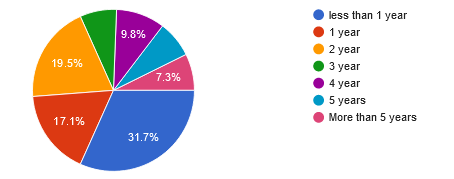
\includegraphics[width=\linewidth]{Images/Experience.png}
    \caption{Google Form Survey participant Years of Experience with solar panel}
    \label{fig:SurveyParticipants}
\end{figure}


\subsection{Data Analysis}
First, the collected data was analyzed carefully. In the solar panel power generation data, April data was missed because of the pandemic situation in Sri Lanka. The whole country went into full lockdown. According to the situation, the electricity board didn't calculate the value for April. This situation created the null value in the data set. At the same time, the 2020 solar panel meter value wasn't collected regularly. It created unnecessary values in the data values. For this reason, the 2020 solar panel dataset was removed from the overall dataset. The solar panel power generation dataset for 2019 was only considered for this research. Using data visualization techniques, the solar panel power generation chart was prepared. Please refer to Figure.~\ref{fig:SolarPowerProduction} to understand how solar panel power production differed according to the month.

\begin{figure}[hbp]
    \centering
    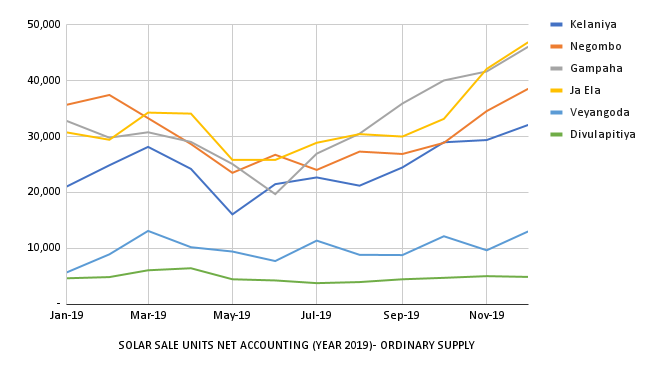
\includegraphics[width=\linewidth]{Images/chart.png}
    \caption{Overall Solar Panel Power Production for 2019 ( Westerns Province - Sri Lanka)}
    \label{fig:SolarPowerProduction}
\end{figure}

At the same time, the weather conditions of 2019 were analyzed to get insights that could help to identify the relationship between solar panel power production and weather conditions. The solar irradiance measurement was missing in the collected weather data. The multiple weather condition charts and the date charts were created using suitable data visualization techniques. Then the weather conditions charts were compared with the solar panel power production chart (Fig.~\ref{fig:SolarPowerProduction}). According to the analysis, the precipitation affects solar panel production directly. The low solar panel power was produced when the high precipitation was monitored by the weather monitoring system.

\begin{figure}[htp]
    \centering
    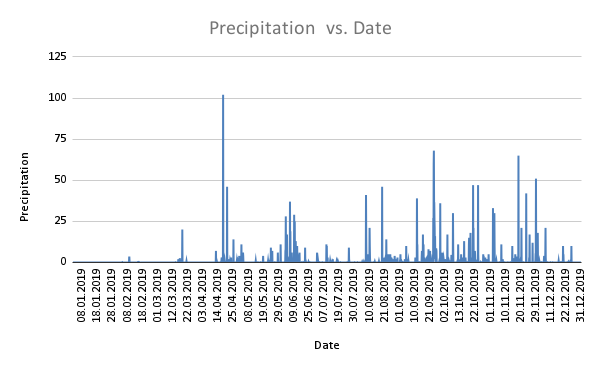
\includegraphics[width=\linewidth]{Images/Precipitation.png}
    \caption{Precipitation of 2019 ( Westerns Province - Sri Lanka)}
    \label{fig:Precipitation}
\end{figure}

\begin{figure}[htp]
    \centering
    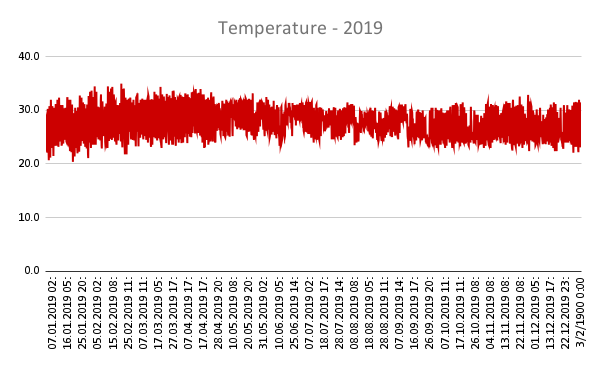
\includegraphics[width=\linewidth]{Images/Temperature - 2019.png}
    \caption{Temperature of 2019 ( Westerns Province - Sri Lanka)}
    \label{fig:Temperature }
\end{figure}


Any liquid or frozen water that develops in the atmosphere and falls back to Earth is referred to as precipitation. Rain, sleet, and snow are just a few examples. \cite{precipitation} According to Sri Lanka, rain is only considered precipitation. The clouds are mostly white. The rain clouds are gray instead of white because of their thickness.  A cloud gets thicker and denser as it gathers more water droplets and ice crystals. The thicker it gets, the more light it scatters, resulting in less light penetrating all the way through it. This reduces the sunlight and causes very low solar power production. The clouds would have more water droplets, be darker, and cause high precipitation in the weather monitoring system. This is the hypothesis that is being considered for this research. 

The temperature affected the solar panel power production by a very small amount. Low-temperature changes were monitored in May, when low solar power was produced. Solar panel power production efficiency can be affected by a few other variables other than the weather conditions like solar radiation and temperature. The factors are 
\begin{itemize}
  \item Solar panel reflection property
  \item Shading from nearby trees or other buildings
  \item Excessive dirt, dust, and pollution
  \item Solar panels are facing direction
\end{itemize}
This research only considered the weather conditions that affect solar panel power production. The dirt, dust, and pollution could reduce solar panel power production. The rain helps to remove the dirt and dust from the solar panels. This creates a sudden increase in solar panel power production after the precipitation has been monitored. In future studies, the effect of dirt, dust, and pollution could be considered in predicting solar panel power production predictions. 

The above analysis confirms that weather conditions like precipitation and temperature affect solar panel power production. The available weather prediction systems like AccuWeather can predict the precipitation and the temperature that affect the solar panel power generation for 10 days \cite{accuweather}. The collected google form data from the experience solar users validate and verify that the weather prediction systems could use to predict solar panel power production. The collected Google form results are shown in Figure 5. 

\begin{figure}[htp]
    \centering
    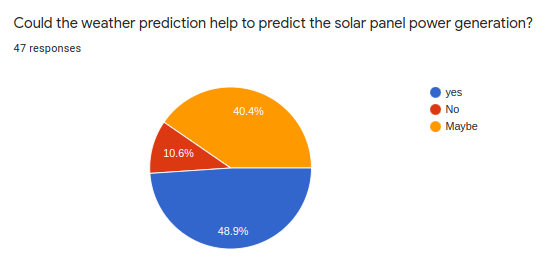
\includegraphics[width=\linewidth]{Images/WeatherPredictionValidation.png}
    \caption{Google Form Survey Result Validate the Weather Prediction System Usage}
    \label{fig:GoogleFormResult }
\end{figure}

The quality attributes like accessibility, usability, reliability, and accuracy of the weather prediction system are evaluated to identify the things that need to be improved in the weather prediction system. The outcome is shown below in Figure.6. The weather prediction systems that provide the predicted weather data for a month won't have good accuracy. This results in low satisfaction with the accuracy of the weather prediction system for the Google form result. 

\begin{figure}[htp]
    \centering
    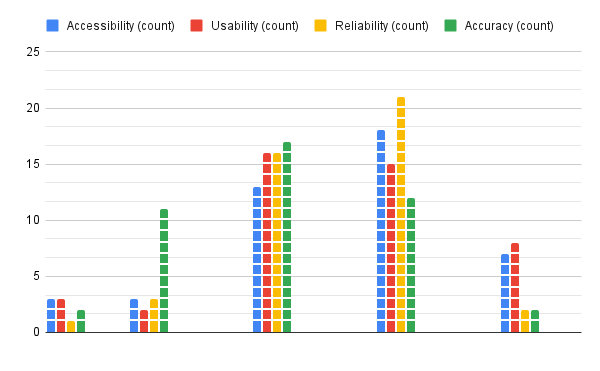
\includegraphics[width=\linewidth]{Images/overall quality.png}
    \caption{Google Form Survey Result About the Weather Prediction System Quality Attributes}
    \label{fig:GoogleFormResult }
\end{figure}

\section{Discussion}

This research shows that temperature and precipitation have a direct impact on solar panel power production. Creating a highly accurate weather prediction system that can predict the temperature and precipitation will help to predict the solar panel power production changes. The solar panel power production system that is created on top of these weather prediction systems can predict the temperature and the precipitation. This system can notify the sudden decrease and increase in solar panel power production to the solar panel users and the interested parties in solar panel power production, like CEB and the industries that depend on solar panel power production.

The notification will help the solar panel users efficiently use the electricity at the low solar power production time. Solar panel users can switch off high-energy-consuming appliances like refrigerators, washing machines, and ovens to save battery power. This helps to reduce the chance of being dependent on the main grid. They can check and confirm that the lithium batteries store electricity at their maximum capacity before the low power production time. Electricity loss can last a few hours to several days in a disaster situation like a storm and heavy rain. The current weather prediction system can be able to predict the storm and heavy rainfall up to 5 days in advance with an accuracy of 90\% \cite{accuracy}. This helps to store the electricity in the lithium batteries before the disaster happens. The stored electricity will help to survive a disaster. This is very helpful to hospitals in saving the patients' lives. 

Electricity producers like CEB can use solar panel power production predictions to assume the demand or load on an electrical main grid. This prediction system can help to implement profitable solar panel energy production in a wide range of energy production.


\section{Conclusion}
This research concludes that temperature and precipitation affect solar panel power production.  The importance and applicability of converting the weather prediction system into the solar panel power prediction system were analyzed. The importance of the solar panel power prediction system to personal and national development was discussed in this research paper.

The future research gap is identified to include more weather conditions like cloud presence and solar panel location factors like dust, dirt, and pollution. The weather forecast accuracy needs to improve. There are various obvious ways to develop upon this analysis proposed in this research.

\section{Acknowledgement}
The support from the Software Engineering Teaching Unit was very helpful to collect the necessary data for this research. The guidance from research supervisor Dr.Lankeswaren was very helpful to complete this research successfully.

% \section{reference}

\bibliographystyle{IEEEtran}
\bibliography{reference}

\end{document}
